\section{Theorie}
\label{sec:Theorie}
Ziel des Versuchs ist die Bestimmung des Kernspins der Rubidium-Isotope $\ce{^{87}Rb}$ und $\ce{^{85}Rb}$.
Dazu wird das optische Pumpen verwendet, wobei durch Hochfrequenz-Strahlung optisch induzierte nicht-thermische Besetzungen erreicht werden.

\subsection{Atomare Quantenzahlen}
Die Elektronenkonfiguration eines Atoms wird beschrieben durch die Hauptquantenzahl $n$, die Bahndrehimpulsquantenzahl $l$ $(0 \leq l < n)$ und die
magnetische Quantenzahl $m$ $(-l \leq m \leq l)$. 
Rubidium gehört zu der Gruppe der Alkali-Metalle und hat die
Elektronenkonfiguration $[Kr]\,5s^1$. 
Da die Alkali-Metalle nur ein Elektron in einer unabgeschlossenen Schale besitzen, können diese gut durch ein ein-Elektron-Atom Modell genähert werden.
In einfachster Darstellung ist die Energie dieser ein-Elektron-Atome nur von der Hauptquantenzahl abhängig, jedoch gibt es auch kleinere Energiekorrekturen
auf die im folgenden eingegangen wird. Die Energieaufspaltungen der Niveaus der folgenden Korrekturen ist in Abbildung \ref{pic:en} dargestellt.
\begin{figure}
    \centering
    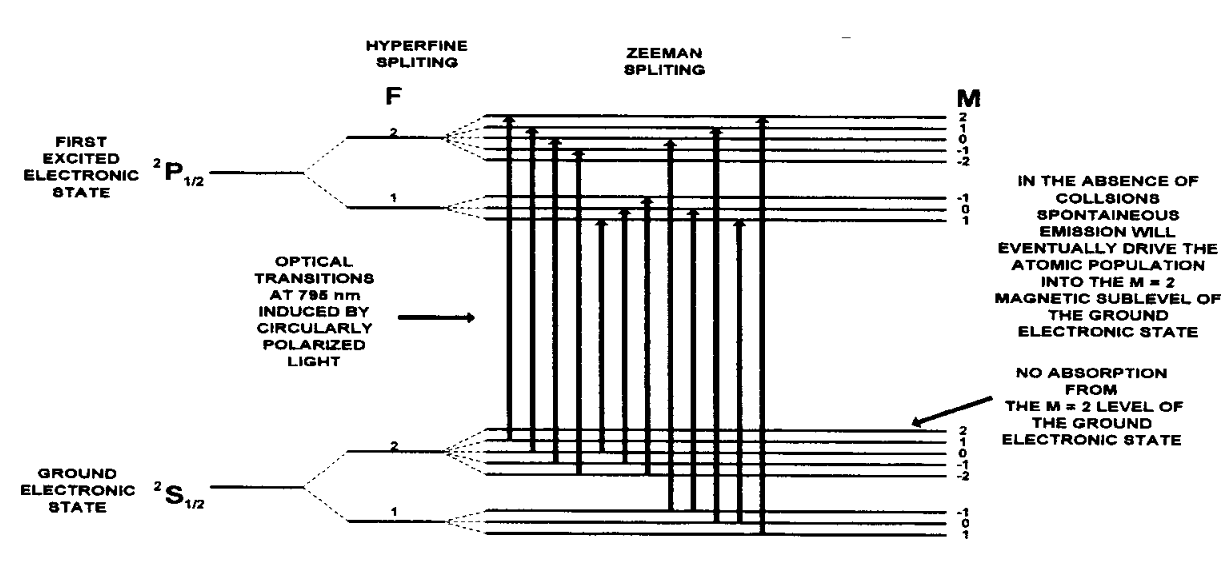
\includegraphics[width = 0.78\textwidth]{pics/energielevel.png}
    \caption{Aufspaltung der Energieniveaus des $^2S_{\frac{1}{2}}$ und des $^2P_{\frac{1}{2}}$ Zustands durch die drei Effekte.\cite{Optisches pumpen}}
    \label{pic:en}
\end{figure}

\subsubsection{LS-Kopplung}
Das Elektron verspürt im Ruhesystem ein Magnetfeld, welches durch den geladenen Kern induziert wird der sich um das Elektron bewegt.
Wird dem Modell der Spin des Elektrons hinzugefügt, spalten die vorherigen Energieniveaus nach dem jeweiligen Gesamtdrehimpuls auf.
Der Gesamtdrehimpuls $J$ setzt sich aus dem Bahndrehimpuls und dem Spin der Hüllenelektronen zusammen und geht von $|L - S|$ bis $|L + S|$.
In dem Grundzustand ergibt sich für beide Isotope $J = S =$\sfrac{1}{2}, da nur ein Hüllenelektron vorhanden ist.

\subsubsection{Hyperfeinstruktur}
Eine deutlich geringere Aufspaltung resultiert aus der Wechselwirkung der Elektronen mit den magnetischen Momenten der Kerne.
Dafür wird eine neue Gesamtdrehimpuls Quantenzahl $F$ eingeführt, welche von $|I - J|$ bis $|I + J|$ läuft mit dem Kernspin $I$.
Der Kernspin $I$ setzt sich aus den Spins der Protonen und Neutronen im Kern zusammen, sodass sich für $\ce{^{85}Rb}$ $I = $ \sfrac{5}{2} und für $\ce{^{87}Rb}$
$I = $\sfrac{3}{2} ergibt. Die Energieniveaus spalten sich nach den neuen Gesamtdrehimpulsen $F$ auf. 

\subsubsection{Der Zeemann-Effekt}
Durch ein externes Magnetfeld kann eine weitere Aufspaltung durch den Zeemann-Effekt erreicht werden.
Dabei wechselwirken das magnetische Moment des Atoms und das Magnetfeld miteinander, wodurch die Aufspaltung in die
verschiedenen Orientierungen des Gesamtdrehimpulses $M_F$ ($-F \leq M \leq F$) entsteht. Für diesen Versuch wird ein starkes magnetisches Feld benötigt,
weshalb der quadratische Zeemann-Effekt betrachtet wird.
Durch Störungstheorie ergibt sich der Energieunterschied
\begin{equation}
    \symup{\Delta} E_Z = g_F \mu_B B + (g_F \mu_B B)^2 \frac{1-2M_F}{\symup{\Delta} E_{Hyp}}
\end{equation}
zwischen dem Grundniveau der Hyperfeinstruktur und dem Energielevel mit magnetischer Quantenzahl $M_F$. 
$\symup{\Delta} E_{Hyp}$ beschreibt hier die Energieaufspaltung zwischen zwei Niveaus der Hyperfeinstruktur mit Gesamtdrehimpuls $F$ und $F+1$.
Des weiteren ist $\mu_B = $\sfrac{$e \hbar$}{$2m_e$} das Bohrsche Magneton und $g_F$ das gyromagnetische Verhältniss, welches durch
\begin{equation}
    g_F = g_J \frac{F(F+1)+J(J+1)-I(I+1)}{2F(F+1)}
\end{equation}
mit
\begin{equation}
    g_J = \frac{J(J+1)+S(S+1)-L(L+1)}{2J(J+1)}
\end{equation}
berechnet werden kann.

\subsection{Optisches Pumpen}
\begin{figure}
    \centering
    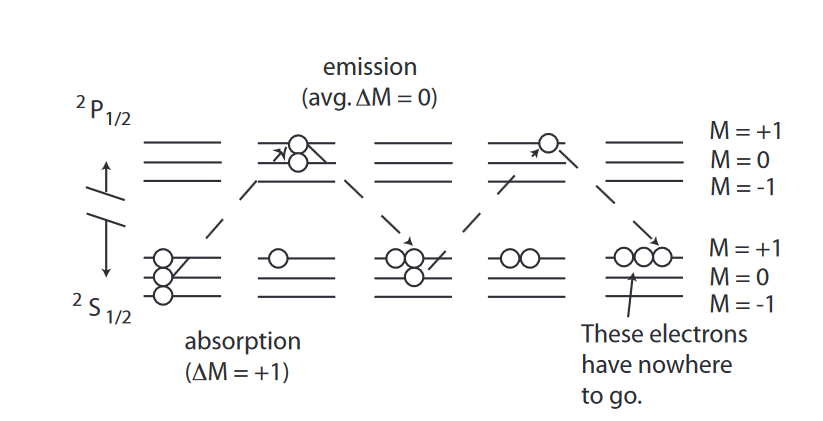
\includegraphics[width = 0.78\textwidth]{pics/pumpen.png}
    \caption{Schematische Darstellung des optischen Pumpens am Wasserstoffatom.\cite{Optisches pumpen}}
    \label{pic:pump}
\end{figure}
In Abbildung \ref{pic:pump} wird das optische Pumpen schematisch am Wasserstoffatom dargestellt.

Bei der An-/Abregung eines Elektrons sind nur Übergänge möglich welche der Auswahlregel $\symup{\Delta{M_F}} = 0, \pm 1$ gehorchen.
Dabei tritt bei spontaner Emission ein zufälliges $\symup{\Delta{M_F}}$ auf. Bei Anregung durch Licht ist die Polarisation entscheidend.
rechtszirkular-polarisiertes Licht erzeugt Übergänge mit $\symup{\Delta{M_F}} = +1$, linkszirkulares mit $\symup{\Delta{M_F}} = -1$ und linear polarisiertes
mit $\symup{\Delta{M_F}} = 0$.

Die Energiedifferenzen, welche durch die Hyperfeinstruktur und den Zeemann-Effekt auftreten, sind klein genug um die Niveaus bei Raumtemperatur als Äquivalent anzusehen.
Wird also auf ein Atom rechts-polarisiertes Licht, welches der Energie des D1-Übergangs entspricht, gestrahlt und ein Magnetfeld entlang der selben Richtung angelegt, kommt es zuerst zu einer Absorption mit $\symup{\Delta{M_F}} = +1$.
Die Absorption kann nur unter dieser Bedingung stattfinden, sodass Elektronen welche kein höheres $M_F$ erreichen können kein Photon absorbieren können.
Bei Emissionsevents kommt es im Durchschnitt zu $\symup{\Delta{M_F}} = 0$. Da auch photonen emittiert werden von einem Übergang mit $\symup{\Delta{M_F}} = -1$, können diese zu
stimulierter Emission führen. Aufgrund der statistischen Verteilung der magnetischen Quantenzahlen wird dennoch nach mehrfachen wiederholen von Absorption und Emission ein Zustand erreicht
in dem sich alle Elektronen in dem Grundzustand mit dem höchsten Wert für $M_F$ befinden. Da nun keine Absorption mehr stattfinden kann, wirkt das Gas durchsichtig für das Licht und wird als polarisiert bezeichnet.
Bei entfernen des Magnetfeldes oder der Lichtquelle wird die Polarisation des Gases verschwinden. Entspricht die Energie der Photonen genau der Energiedifferenz der Zeemann-Aufspaltung kommt es zu
Resonanz und die stimulierte Emission steigt. Es bildet sich ein Gleichgewicht, sodass das polarisierte Gas bei der Resonanz an Transparenz verliert.
Dies kann zum Beispiel wie in Abbildung \ref{pic:resonanz} über das variieren des Magnetfelds erreicht werden. Die Resonanz tritt dann bei einem Magnetfeld von 
\begin{equation}
    B_m = \frac{\hbar \omega_{RF}}{g_F \mu_B}
\end{equation}
auf.
\begin{figure}
    \centering
    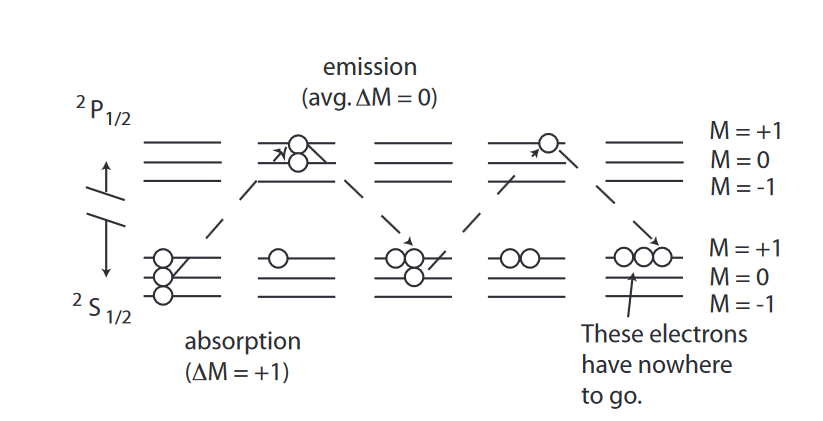
\includegraphics[width = 0.78\textwidth]{pics/pumpen.png}
    \caption{Transparenz eines polarisierten Gases in Abhängigkeit vom Magnetfeld.\cite{V21}}
    \label{pic:resonanz}
\end{figure}



